\begin{figure}[!htbp]\centering
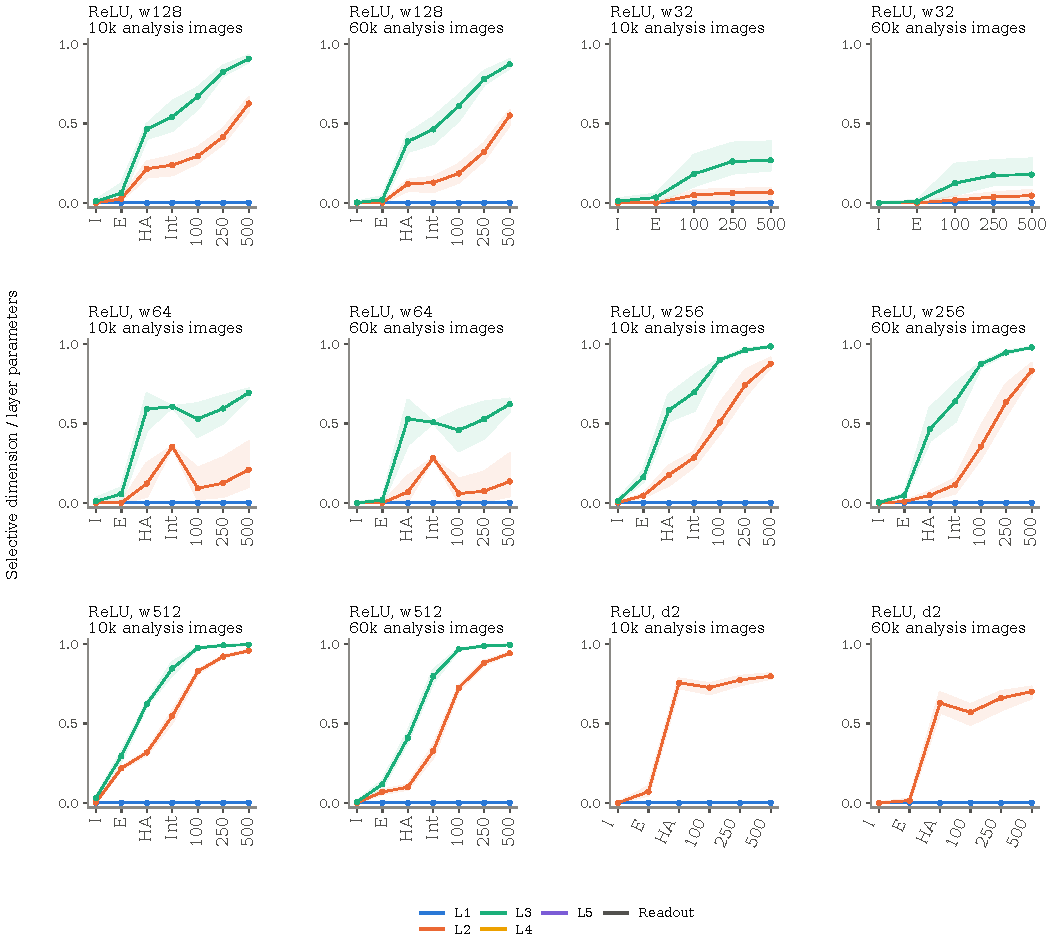
\includegraphics[width=6.315in]{compact_selective_part1.pdf}
\caption{Selective dimension as a fraction of layer parameters, across all tested stages and analysis-set sizes. MNIST is used unless labeled SVHN. Colors identify hidden layers or convolutional layers; lines are seed means and bands span seeds. MLP spaces constrain each unit on its active samples; CNN spaces constrain each channel on its active input patches. A zero identifies an empty selective construction; the full atomic kernel can still contain other directions. Stage abbreviations follow the atomic panels.}
\end{figure}
\begin{figure}[!htbp]\centering
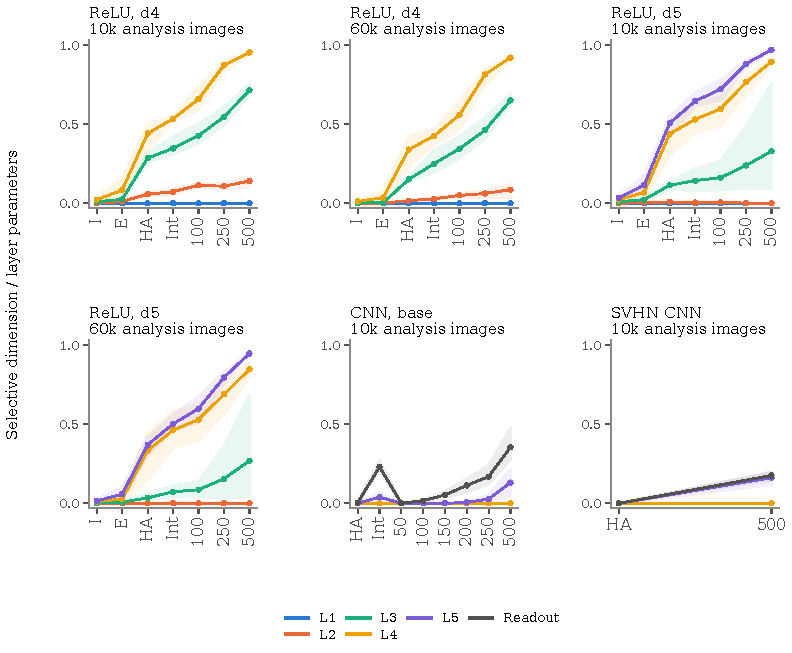
\includegraphics[width=4.754in]{compact_selective_part2.pdf}
\caption{Continued. Selective dimension as a fraction of layer parameters, across all tested stages and analysis-set sizes. MNIST is used unless labeled SVHN. Colors identify hidden layers or convolutional layers; lines are seed means and bands span seeds. MLP spaces constrain each unit on its active samples; CNN spaces constrain each channel on its active input patches. A zero identifies an empty selective construction; the full atomic kernel can still contain other directions. Stage abbreviations follow the atomic panels.}
\end{figure}
\begin{figure}[!htbp]\centering
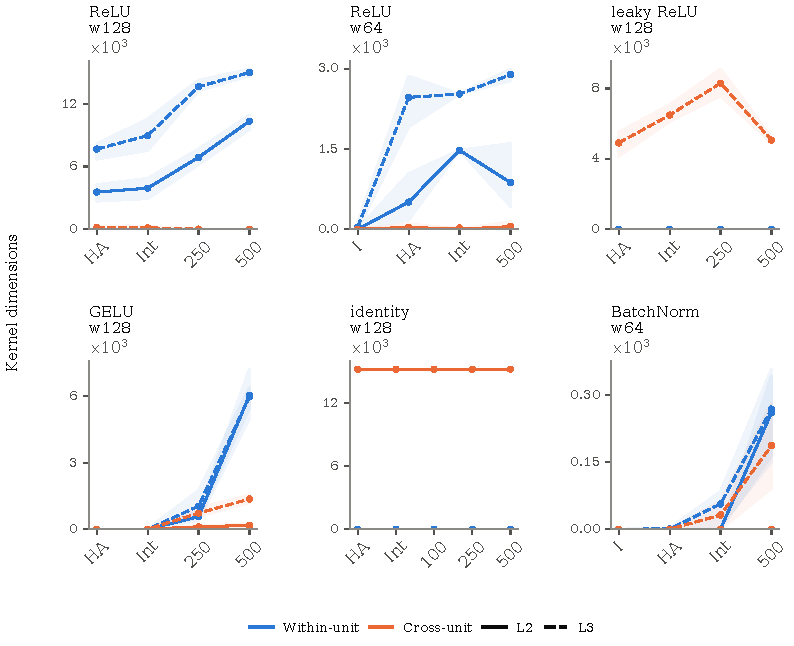
\includegraphics[width=4.762in]{compact_neuron.pdf}
\caption{Within-unit and cross-unit kernel dimensions for MNIST MLPs. Each panel combines L2 and L3, distinguished by line style. Curves are seed means and bands span seeds. ReLU within-unit directions agree with the selective construction where containment checks pass. Leaky-ReLU and GELU per-unit operators use their actual slopes; late GELU counts remain numerical threshold-dependent quantities.}
\end{figure}
\FloatBarrier
